
Prior to the derivation of the expected limits, we have done an optimization study finding the best cut value on the BDT discriminant, which would yield the lowest limit. For this study we optimized electron and muon channels separately. Systematical uncertainties were present only as lnN, since we are statistically limited and not systematics dominated. The latter can be seen running the fit with the "-S 0" option, which ignores systematics entirely. For example, for the 300 GeV fit in the muon channels the 'r-value' with the systematics in is 255.25 (neglecting BBB uncertainties), without systematics it is 238.25. The difference is 17 parts in 255.25, which is just 6.7 $\%$.

\subsection{Obtaining the best limit}

As can be seen from the plots ~\ref{fig:ele_bdt_vs_r} and ~\ref{fig:muon_bdt_vs_r}, for high mass region the best cut to use is 0.99 for both electron and muon channels. For low mass region, the situation is different. Depending on the mass point one cut is better than the other. For electron channel for 400 and 450 GeV the optimal cut is 0.925. Then the situation changes, 0.2 for 260 GeV, 0.4 for 270 and 300 GeV, 0.825 for 350 GeV. Running the whole analysis for each separate cut and channel is not possible computationally taking into account the number of samples and shapes one has to process. That is why a reasonable compromise is to observe that for 260 $\to$ 350 GeV included, the suboptimal cut can be 0.4, being well inside the $1\sigma$ error band. For muons the best cuts are: 0.1 for 260 and 270 GeV, 0.5 for 300 GeV, 0.7 for 350 GeV, 0.925 for 400 and 450 GeV. In this case a suboptimal cuts are: 0.1 for 260 and 270 GeV, 0.7 for 300 $\to$ 450 GeV included. This is summarized in the Table~\ref{suboptCut}:

\begin{table}
\begin{center} 
  \caption{Suboptimal BDT cuts used in the analysis}
 \begin{tabular}{ |c|c|c|c|c| } \hline%\hline
   channel & 260 and 270 GeV & 300 and 350 GeV & 400 and 450 GeV & 600 GeV to 1000 GeV \\ \hline
   muons & 0.1 & 0.7 & 0.7 & 0.99 \\ %\hline
   electrons & 0.4 & 0.4 & 0.925 & 0.99\\ \hline%\hline
  \end{tabular}
  \label{suboptCut}
\end{center}   
\end{table}

This way we simplify the analysis to three different BDT cuts per channel and, at the same time, remain optimal within the error bands with respect  to the best cut values. 

\begin{figure}[!htb]%hbpt?        
\includegraphics[width=0.5\textwidth, height=0.2\textheight,  keepaspectratio]{eles_bdt_vs_r/gr_limits__260GeV.pdf}
\includegraphics[width=0.5\textwidth, height=0.2\textheight,  keepaspectratio]{eles_bdt_vs_r/gr_limits__270GeV.pdf}
\includegraphics[width=0.5\textwidth, height=0.2\textheight,  keepaspectratio]{eles_bdt_vs_r/gr_limits__300GeV.pdf}
\includegraphics[width=0.5\textwidth, height=0.2\textheight,  keepaspectratio]{eles_bdt_vs_r/gr_limits__350GeV.pdf}
\includegraphics[width=0.5\textwidth, height=0.2\textheight,  keepaspectratio]{eles_bdt_vs_r/gr_limits__400GeV.pdf}
\includegraphics[width=0.5\textwidth, height=0.2\textheight, keepaspectratio]{eles_bdt_vs_r/gr_limits__450GeV.pdf}
\includegraphics[width=0.5\textwidth, height=0.2\textheight, keepaspectratio]{eles_bdt_vs_r/gr_limits__600GeV.pdf}
\includegraphics[width=0.5\textwidth, height=0.2\textheight, keepaspectratio]{eles_bdt_vs_r/gr_limits__650GeV.pdf}
\includegraphics[width=0.5\textwidth, height=0.2\textheight, keepaspectratio]{eles_bdt_vs_r/gr_limits__900GeV.pdf}
\hspace{1.9cm}
\includegraphics[width=0.5\textwidth, height=0.2\textheight, keepaspectratio]{eles_bdt_vs_r/gr_limits__1000GeV.pdf}
\caption{ Cut on the BDT output vs 'r-value' from Combine. Electron channel.}
\label{fig:ele_bdt_vs_r}                                                       
\end{figure}



\begin{figure}[!htb]%hbpt?        
\includegraphics[width=0.5\textwidth, height=0.2\textheight, keepaspectratio]{muons_bdt_vs_r/gr_limits__260GeV.pdf}
\includegraphics[width=0.5\textwidth, height=0.2\textheight, keepaspectratio]{muons_bdt_vs_r/gr_limits__270GeV.pdf}
\includegraphics[width=0.5\textwidth, height=0.2\textheight, keepaspectratio]{muons_bdt_vs_r/gr_limits__300GeV.pdf}
\includegraphics[width=0.5\textwidth, height=0.2\textheight, keepaspectratio]{muons_bdt_vs_r/gr_limits__350GeV.pdf}
\includegraphics[width=0.5\textwidth, height=0.2\textheight, keepaspectratio]{muons_bdt_vs_r/gr_limits__400GeV.pdf}
\includegraphics[width=0.5\textwidth, height=0.2\textheight, keepaspectratio]{muons_bdt_vs_r/gr_limits__450GeV.pdf}
\includegraphics[width=0.5\textwidth, height=0.2\textheight, keepaspectratio]{muons_bdt_vs_r/gr_limits__600GeV.pdf}
\includegraphics[width=0.5\textwidth, height=0.2\textheight, keepaspectratio]{muons_bdt_vs_r/gr_limits__650GeV.pdf}
\includegraphics[width=0.5\textwidth, height=0.2\textheight, keepaspectratio]{muons_bdt_vs_r/gr_limits__900GeV.pdf}
\hspace{1.9cm}
\includegraphics[width=0.5\textwidth, height=0.2\textheight, keepaspectratio]{muons_bdt_vs_r/gr_limits__1000GeV.pdf}
\caption{ Cut on the BDT output vs 'r-value' from Combine. Muon channel.}
\label{fig:muon_bdt_vs_r}           
\end{figure}

 
\subsection{Results from the fit}
Binned shape analysis is performed using Higgs Combination Tool  \cite{HiggsCombine}.  

We do a simultaneous fit (HH transverse mass distribution is used) of all three
regions - signal region and two control regions, to extract both
signal strength parameter as well as normalizations of \ttbar and
Drell-Yan backgrounds.  We use the following command:  \hfill \break
$\textit{combine 
-M Asymptotic -t -1 -v 3 -m massValue --run blind
comb\_card\_massValue.txt}$.


%Vertical lines as column separators
\begin{table}
\begin{center}
\caption{Normalization for backgrounds, final numbers after the application of all the nuisances during the postfit procedure. Electron channel.}
\begin{tabular}{ | c | c | c | }
  \hline
  channel,mass & TT\_SF & DY\_SF \\
  \hline
  ee 300 GeV    & 0.80 +/- 0.09   &  1.62 +/- 0.23\\
  ee 900 GeV    & 0.79 +/- 0.08    & 1.64 +/- 0.18\\
  \hline
\end{tabular}
\label{normalization_electron}
\end{center}
%---------------------------------------------------------------------
%Vertical lines as column separators
\begin{center}
\caption{Normalisation for backgrounds in the unblinded SR, final numbers after the application of all the nuisances during the postfit procedure. Electron channel.}
\begin{tabular}{ | c | c | c | }
  \hline
  channel,mass & TT\_SF & DY\_SF \\
  \hline
  ee 300 GeV    &  0.8 +/- 0.1    &   1.58 +/- 0.25 \\
%fit_s
 ee 900 GeV    &  0.9 +/- 0.33     &  1.75 +/- 0.49\\
%from  log_PostFitShapesFromWorkspace_ee_SR_hhMt_FullPostfit.txt
  \hline
\end{tabular}
\label{normalization_electron_SR}
\end{center}
\end{table}
%---------------------------------------------------------------------


%\vspace{1cm}
\begin{table}
\begin{center}
\caption{Normalization for backgrounds, final numbers after the application of all the nuisances during the postfit procedure. Muon channel.}
\begin{tabular}{ | c | c | c | }
  \hline
  channel,mass & TT\_SF & DY\_SF \\
  \hline
  mm 300 GeV   & 0.91 +/- 0.07 & 1.44 +/- 0.13\\
  mm 900 GeV   & 0.91 +/- 0.07 & 1.43 +/- 0.13\\

  \hline
\end{tabular}
\label{normalization_muon}
\end{center}
%\vspace{1cm}
\begin{center}
\caption{Normalisation for backgrounds in the unblinded SR, final numbers after the application of all the nuisances during the postfit procedure. Muon channel.}

\begin{tabular}{ | c | c | c | }
  \hline
  channel,mass & TT\_SF & DY\_SF \\
  \hline
  mm 300 GeV   &  0.91 +/- 0.07  & 1.49 +/- 0.15\\
  mm 900 GeV   &  0.91 +/- 0.19  & 1.53 +/- 0.42\\

  \hline
\end{tabular}
\label{normalization_muon_SR}
\end{center}
\end{table}

%% \begin{table}
%% \begin{center}
%%   \caption{Normalization for backgrounds, which were extracted from the simultaneous fit of all regions. Muon channel.}
%%  \begin{tabular}{ |c|c|c| } \hline%\hline
%%    Mass & Drell-Yan normalization & \ttbar normalization \\ \hline
%%    300 GeV & 1.3675e+00         +/-  7.85e-02  & 1.0969e+00         +/-  8.23e-02 \\
%%    900 GeV & 1.3866e+00         +/-  1.42e-01  & 8.6785e-01         +/-  1.04e-01 \\ \hline%\hline
%%   \end{tabular}
%%   \label{normalization_muon}
%% \end{center}
%% \end{table}




%% Here are limits explicitly for one mass point in the low mass region and one mass point in the high mass region.

%% \begin{table}
%% \begin{center}
%% \caption{Expected limits for 300 and 900 GeV for electron, muon, and combined channels.}
%% \label{combLimits}
%% \begin{tabular}{ |c|c|c|  }
%%  \hline
%%  %\hline
%% Channel & 300 GeV & 900 GeV\\
%%  \hline         
%% electron & Expected 50.0\%: r $<$ 433.75 & Expected 50.0\%: r $<$ 3.859\\
%% muon & Expected 50.0\%: r $<$ 255.25 & Expected 50.0\%: r $<$ 3.734\\
%% combined & Expected 50.0\%: r $<$ 218.25 & Expected 50.0\%: r $<$ 2.30\\
%%  \hline %\hline
%% \end{tabular}
%% \end{center}
%% \end{table}




%% \begin{table}
%% \begin{center}
%%  \caption{Normalization for backgrounds, which were extracted from the simultaneous fit of all regions. Electron channel.}
%%  \begin{tabular}{ |c|c|c| }\hline%\hline 
%%          Mass & Drell-Yan normalization & \ttbar normalization \\  \hline 
%%        300 GeV & 1.4678e+00         +/-  8.13e-02 & 9.4753e-01         +/-  6.99e-02\\ 
%%        900 GeV & 1.7415e+00         +/-  1.88e-01 & 8.0511e-01         +/-  1.04e-01 \\ \hline%\hline
%%  \end{tabular}
%%   \label{normalization_electron}
%% \end{center}
%% \end{table}





%% \begin{table}
%% \begin{center}
%%   \caption{Normalization for backgrounds, which were extracted from the simultaneous fit of all regions. Combined data.}
%%  \begin{tabular}{ |c|c|c| } \hline%\hline
%%    Mass & Drell-Yan normalization & \ttbar normalization \\ \hline
%%    300 GeV & 1.3537e+00         +/-  1.28e-01  &   9.4549e-01         +/-  1.06e-01 \\
%%    900 GeV & 1.4974e+00         +/-  1.48e-01  & 8.4310e-01         +/-  1.02e-01\\
%% \hline%\hline
%%   \end{tabular}
%%   \label{normalization_comb}
%% \end{center}
%% \end{table}





The limits in the Table ~\ref{finalLimits} are showing the results for combined data using electron and muon channels. The corresponding plots are shown on the Figs. ~\ref{fig:HHlimits}. %Separately limits for electron and muon channels are shown at the Figs. ~\ref{fig:HHlimits}. 
The values of the DY and \ttbar normalizations in control regions extracted during the simultaneous fit of signal and control regions are shown in the Tables ~\ref{normalization_electron}, ~\ref{normalization_muon}.%, and ~\ref{normalization_comb}. 
Full postfit distributions (the naming emphasizes all regions are used in the fit, signal region included) are shown on the Figs. ~\ref{fig:MCcomparisons} for the graviton case and ~\ref{fig:MCcomparisons_radion} for the radion case. 
%Comprehensive study with per channel distributions and for different mass regions can be found on Figs. ~\ref{fig:MCcomparison_mm_300} - ~\ref{fig:MCcomparison_ee_900}.


The corresponding values of the DY and \ttbar normalizations in the unblinded SR control regions are shown in the Tables ~\ref{normalization_electron_SR}, ~\ref{normalization_muon_SR}.






%% \begin{figure}[!htb]%hbpt?                                                                                                      
%%   \begin{center}                                                                                                                        
%% %    \raisebox{0.17\height}                                                                                                              
%%     %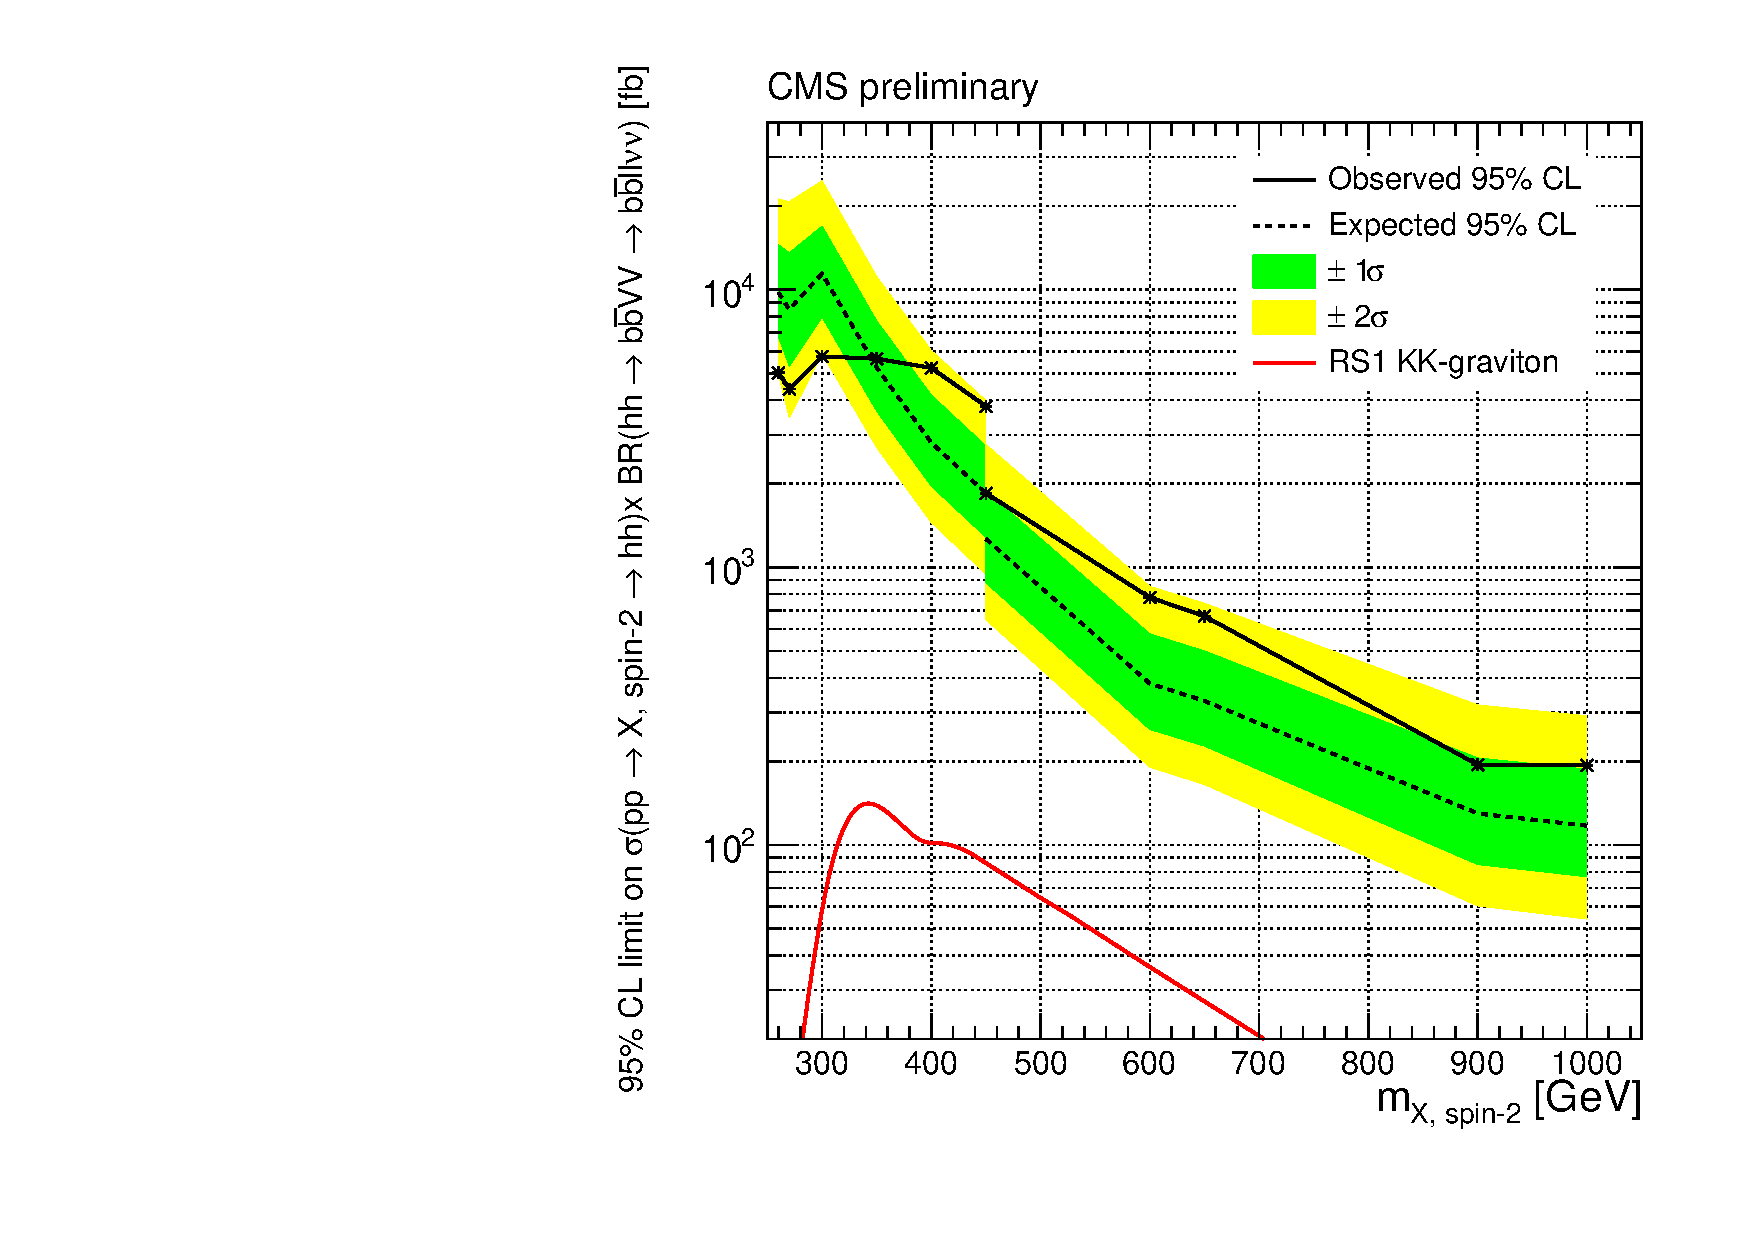
\includegraphics[width=0.65\textwidth]{limitbbZZ_apr29_comb.pdf}                                                                                 
%%     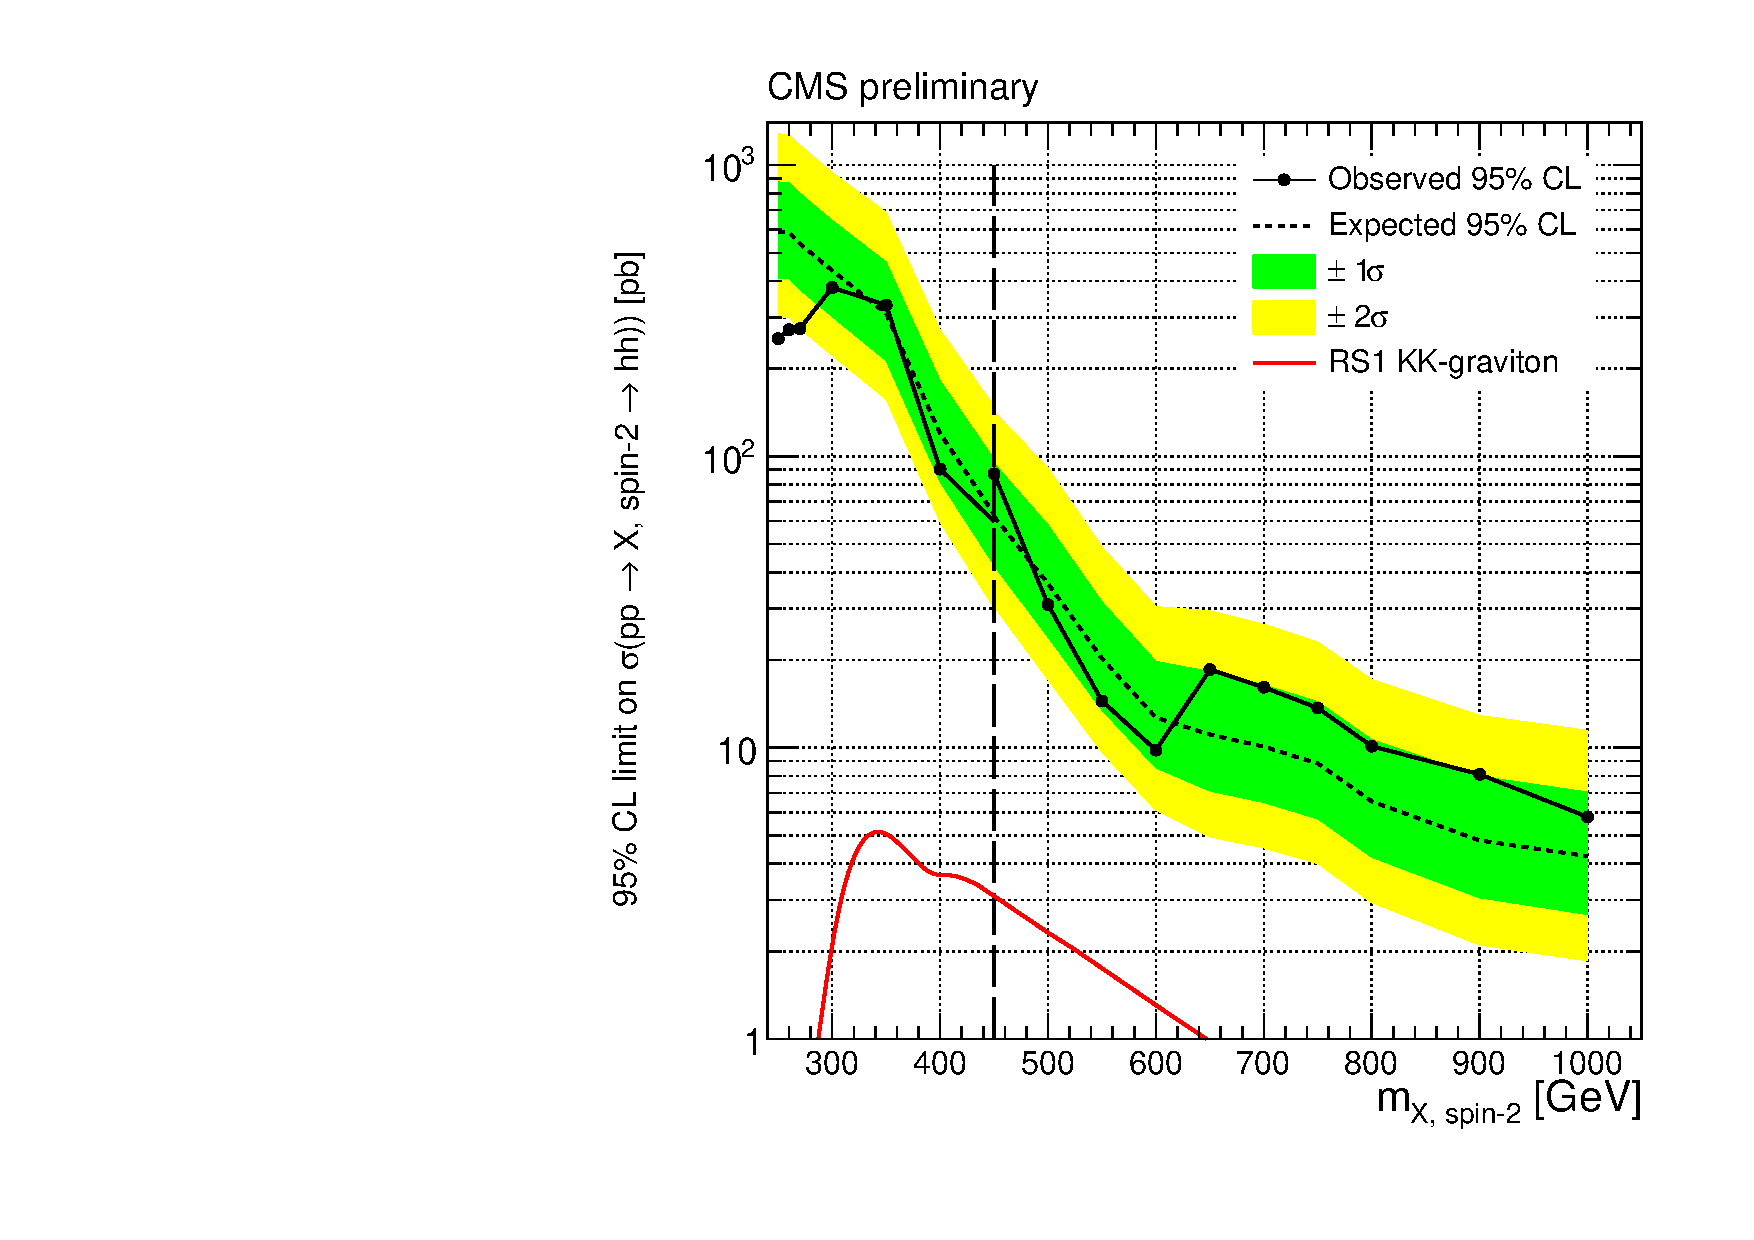
\includegraphics[width=0.65\textwidth]{limitHH_July16_comb.pdf}                                                                                    
%%     \caption{ Expected and observed limits on the HH production. %Top: in the 2 b jets, 2 lepton, 2 neutrinos final state optimized for the bbZZ selection. Bottom: full HH production. 
%%     }                                                                                                                                   
%%     \label{fig:bbZZlimits}                                                                                                                  
%%   \end{center}                                                                                                                          
%% \end{figure}



%% \begin{figure}[!htb]%hbpt?                                                                                                              
%%   \begin{center}                                                                                                                        
%%     %\raisebox{0.17\height}                                                                                                              
%%   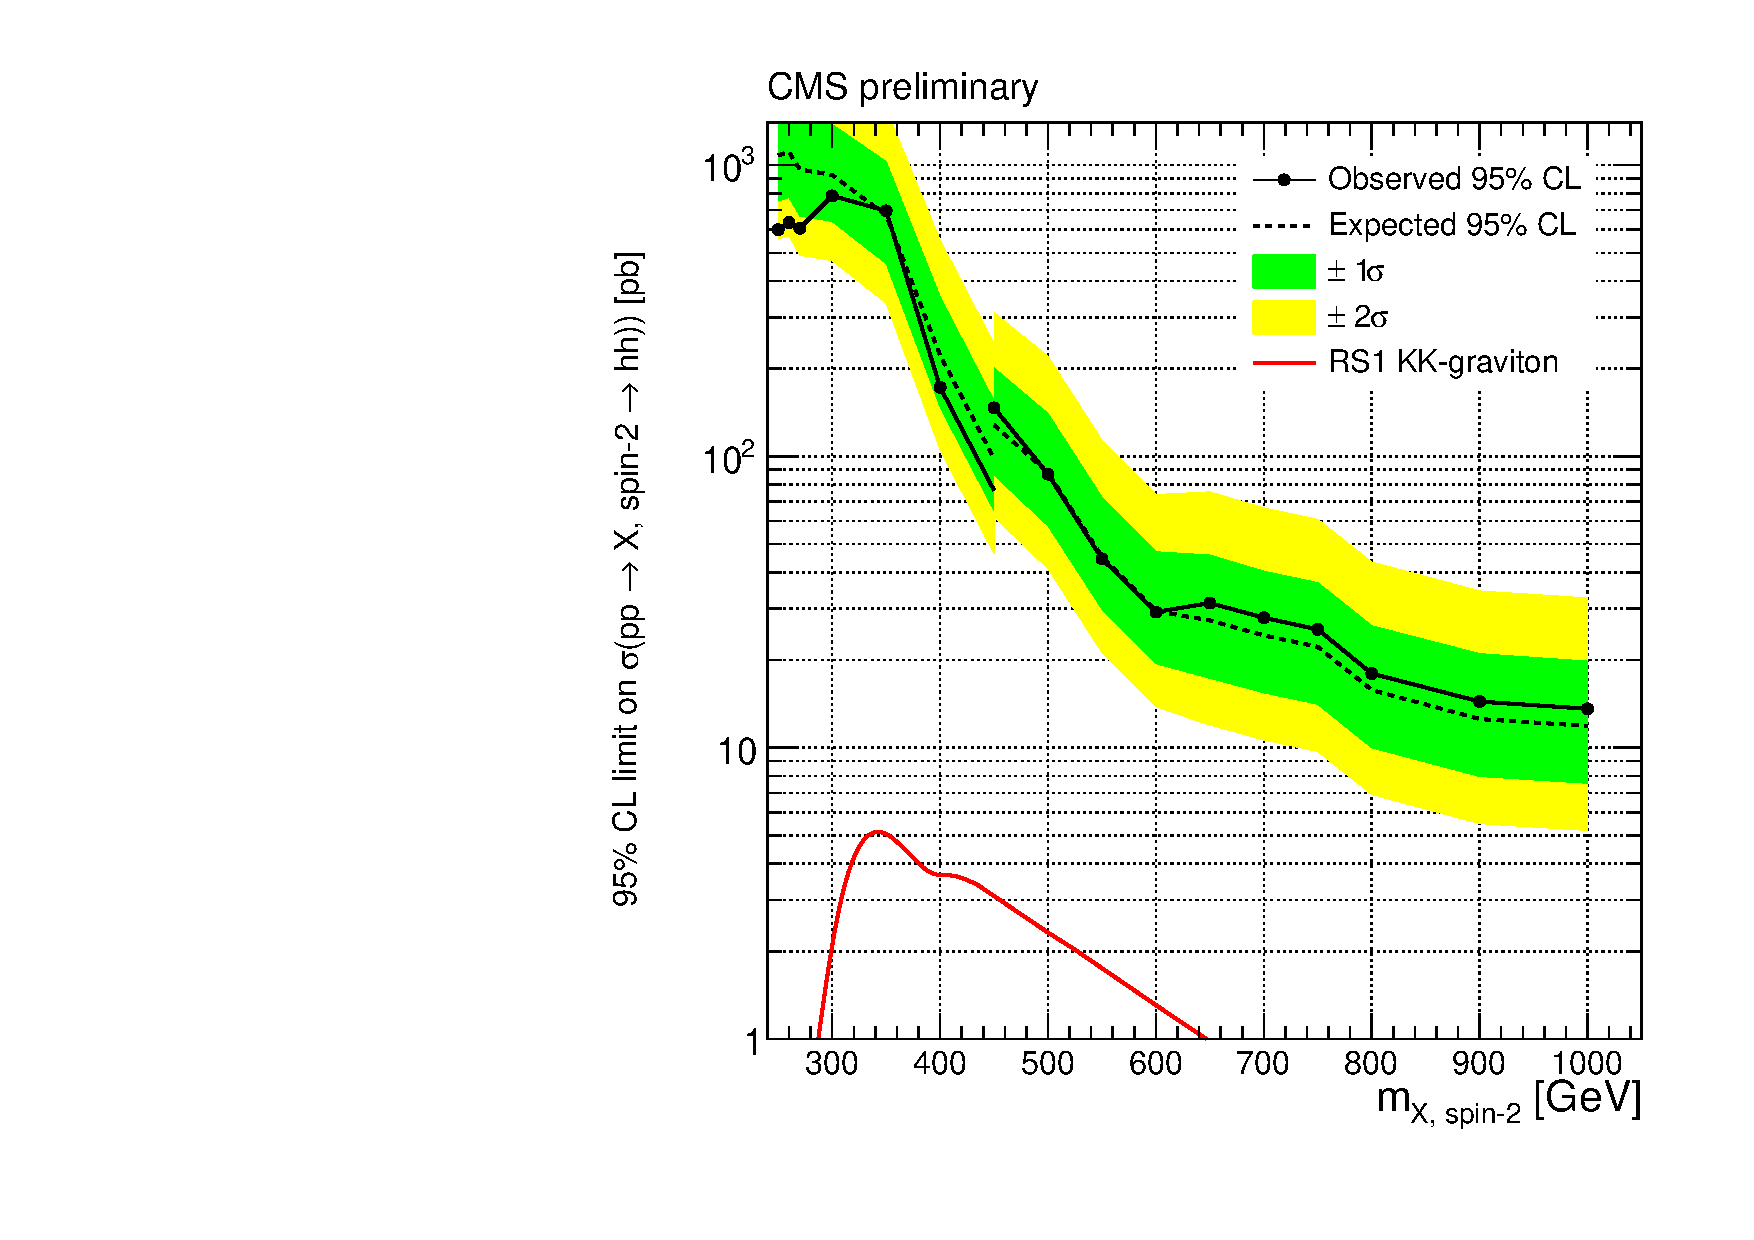
\includegraphics[width=0.65\textwidth]{limitHH_July16_ee.pdf} 
%%   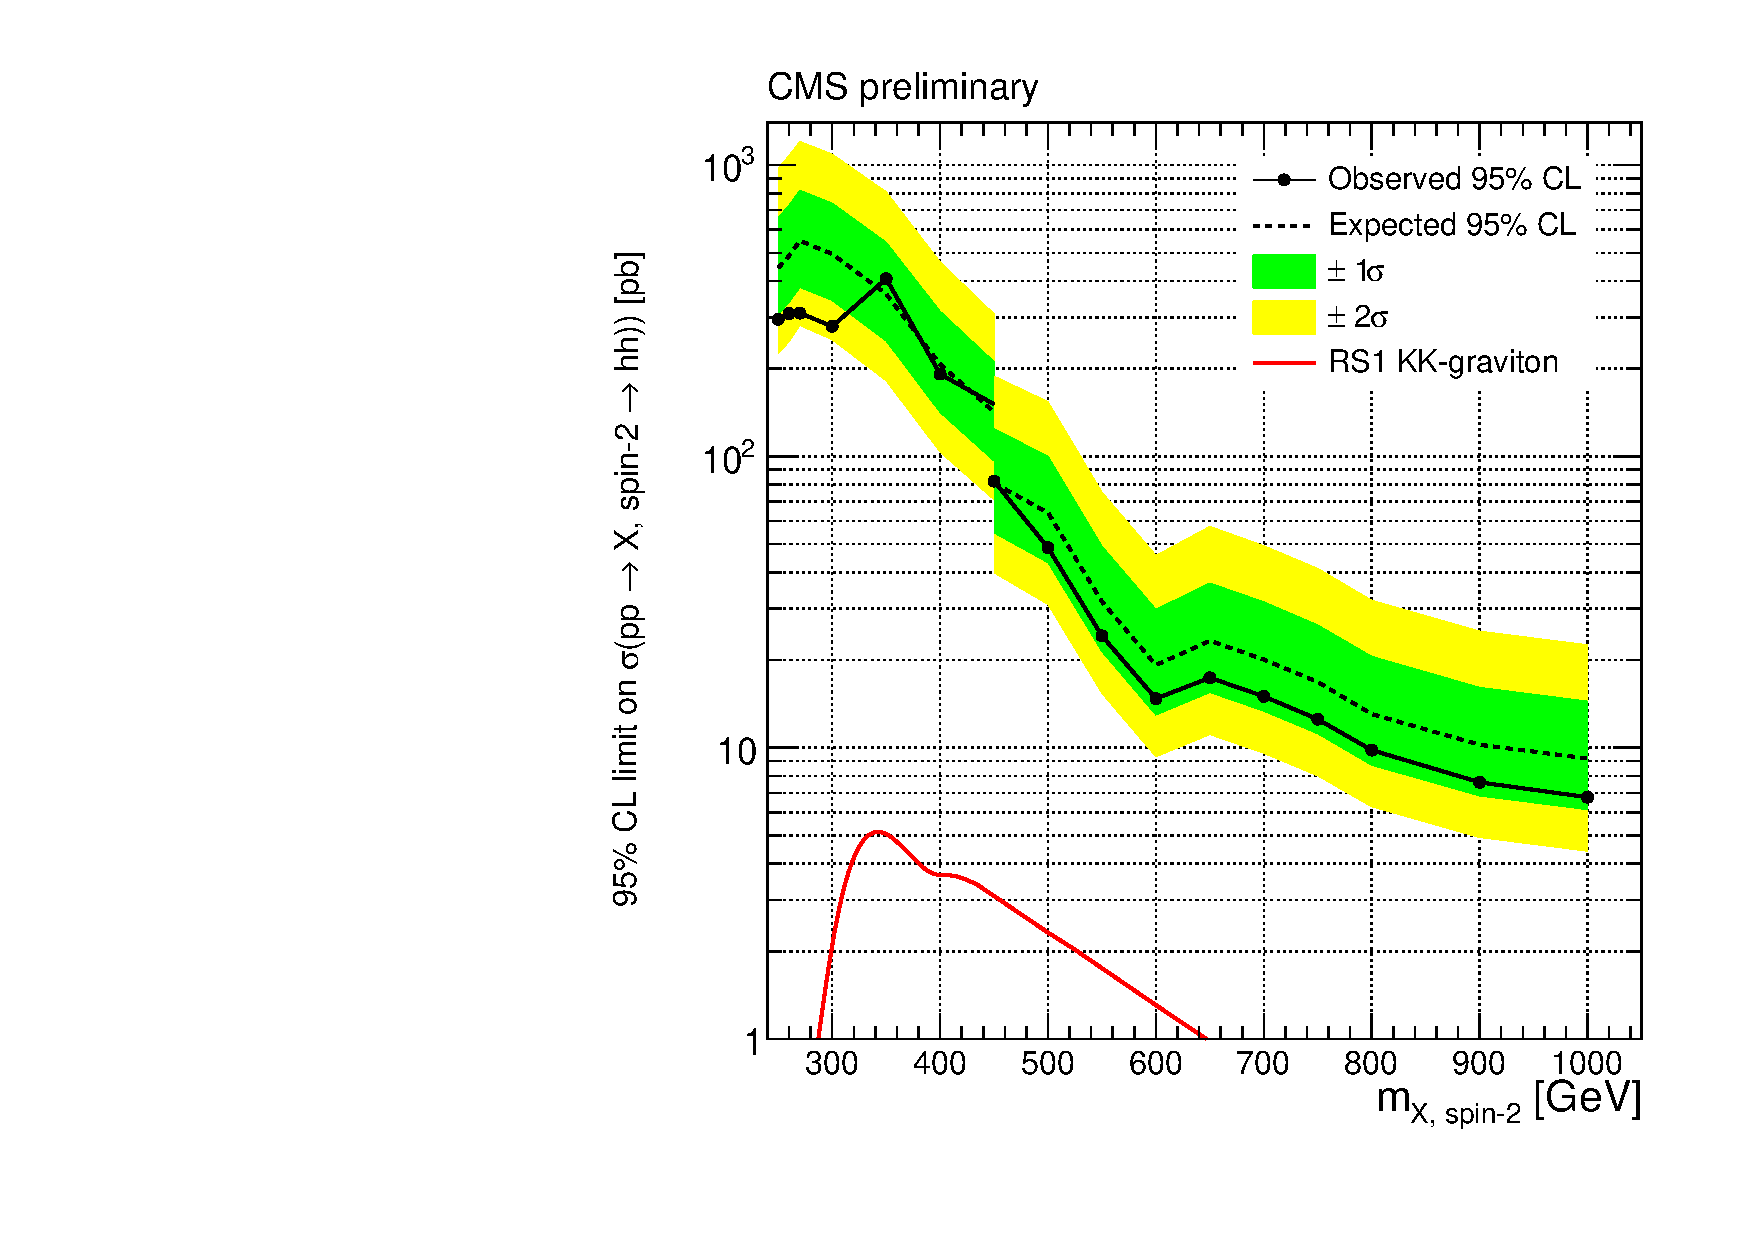
\includegraphics[width=0.65\textwidth]{limitHH_July16_mm.pdf}                                                              
%%   \caption{ Expected and observed limits on the full HH production. Top: electron channel. Bottom: muon channel.     }                      
%%   \label{fig:HHlimits}                                                                                                                  
%%   \end{center}                                                                                                                          
%% \end{figure}


\begin{figure}[!htb]%hbpt?                                                                                        
  \begin{center}
%    \raisebox{0.17\height}                                                                                       
    %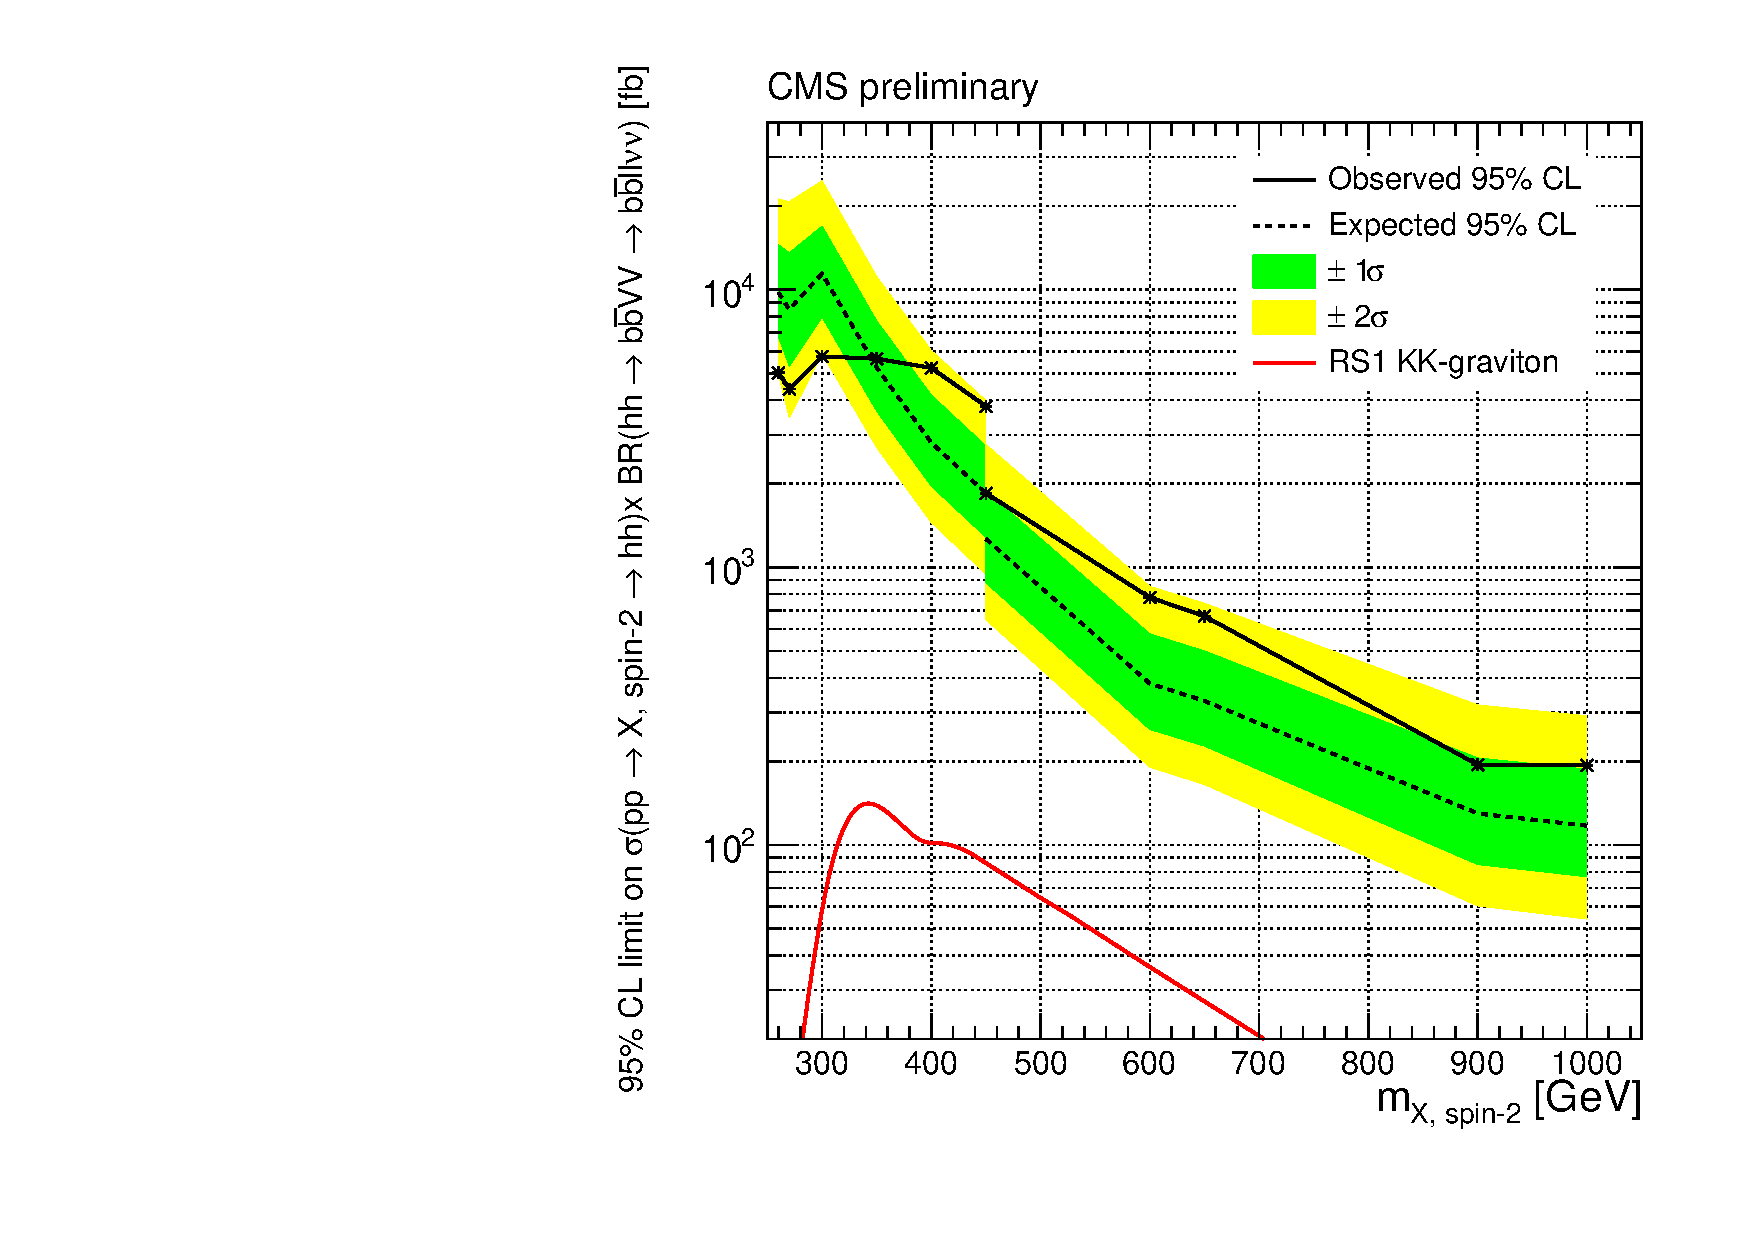
\includegraphics[width=0.65\textwidth]{limitbbZZ_apr29_comb.pdf}                                     
    %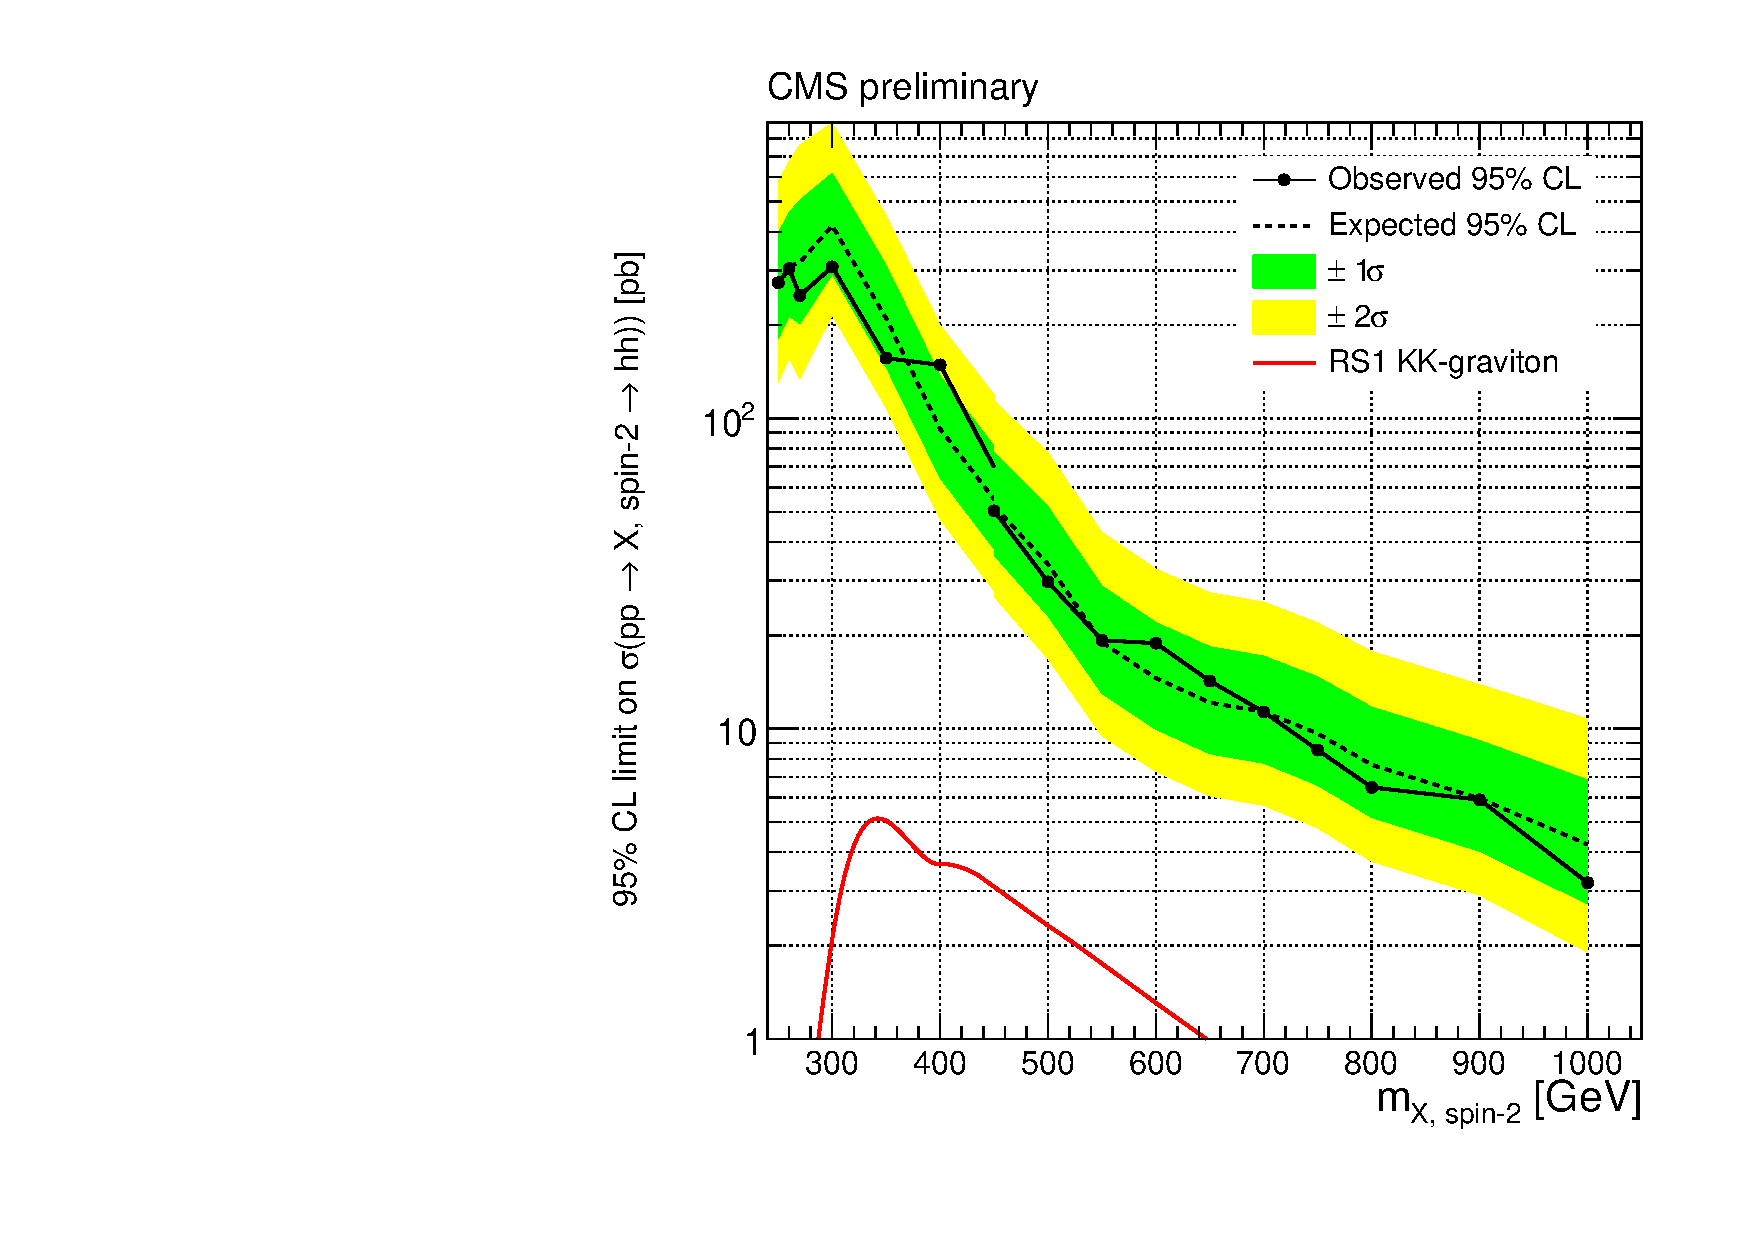
\includegraphics[width=0.65\textwidth]{limitHH_June13_comb.pdf}                                      
    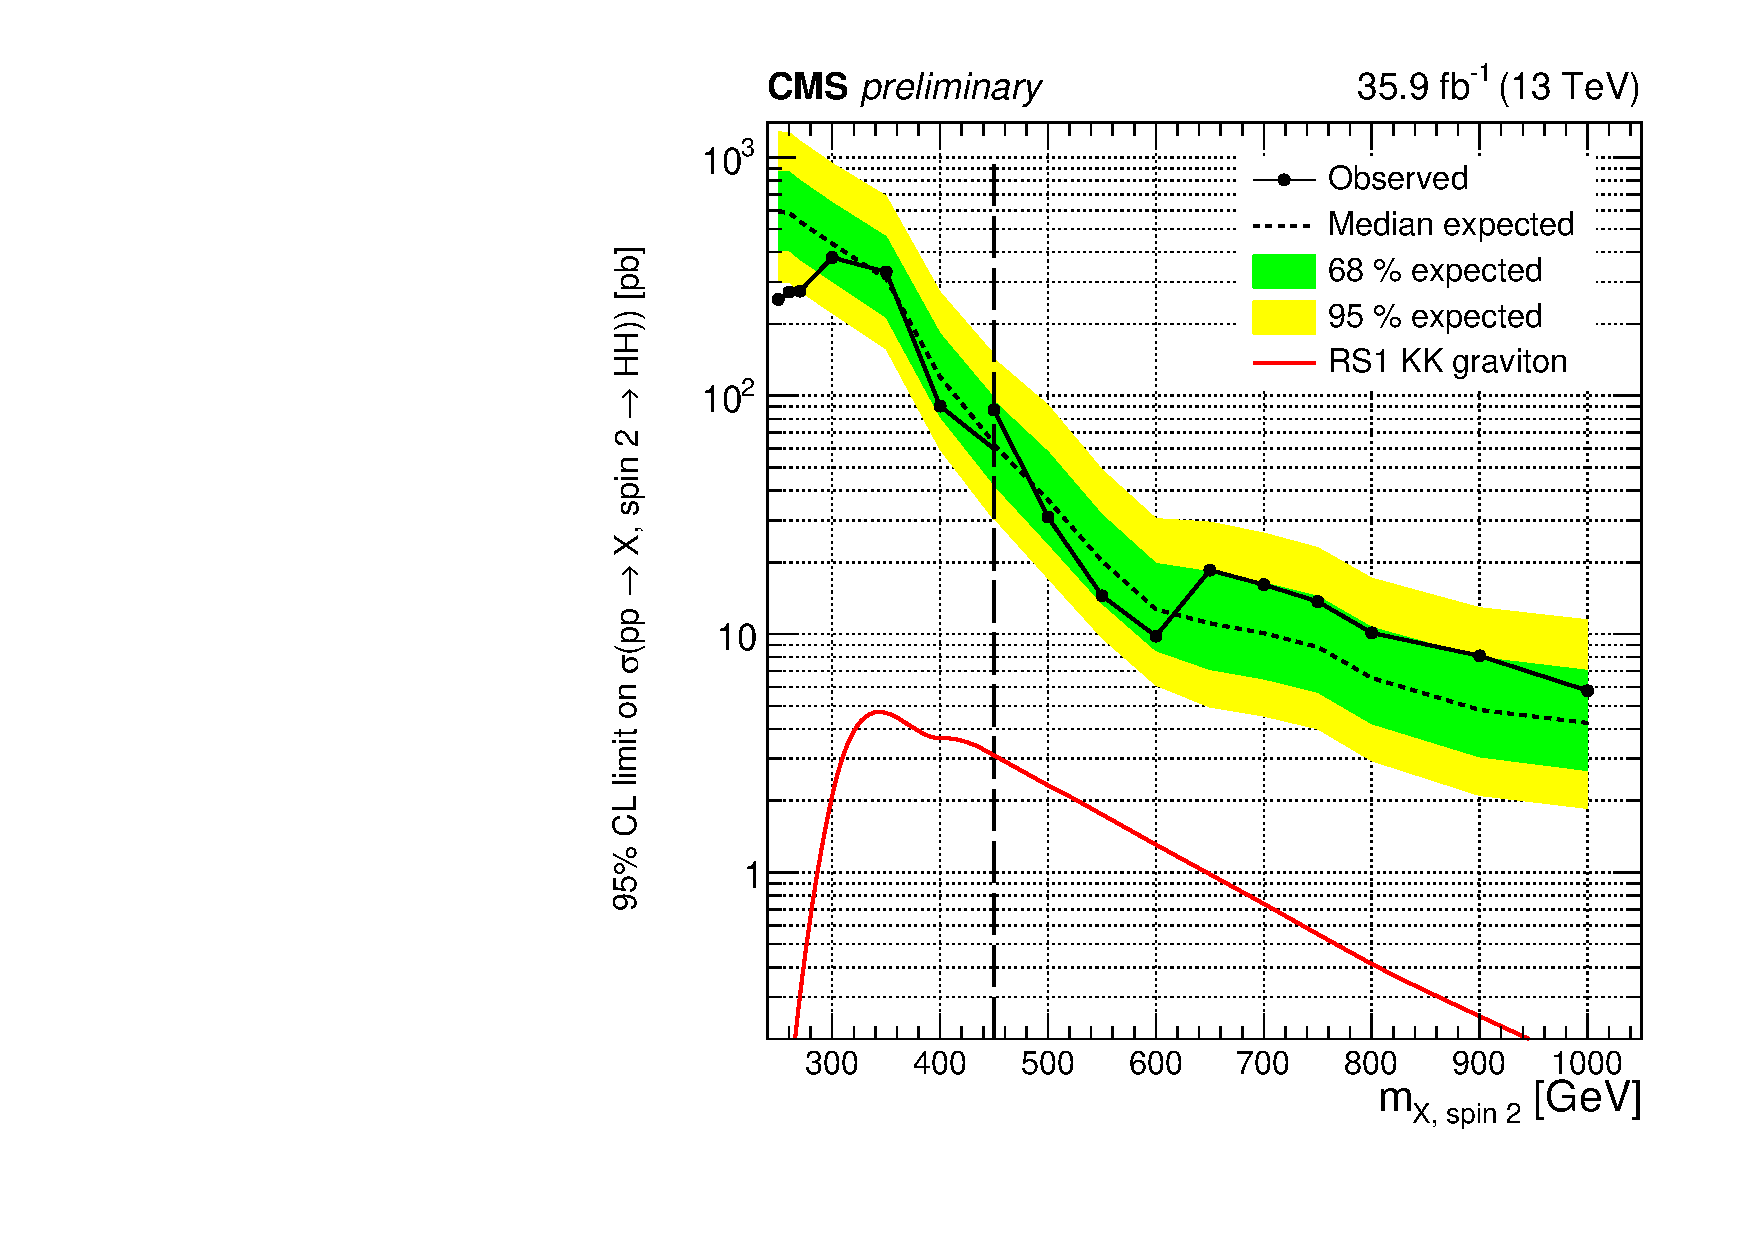
\includegraphics[width=0.65\textwidth]{limitHH_Nov16_graviton.pdf}
    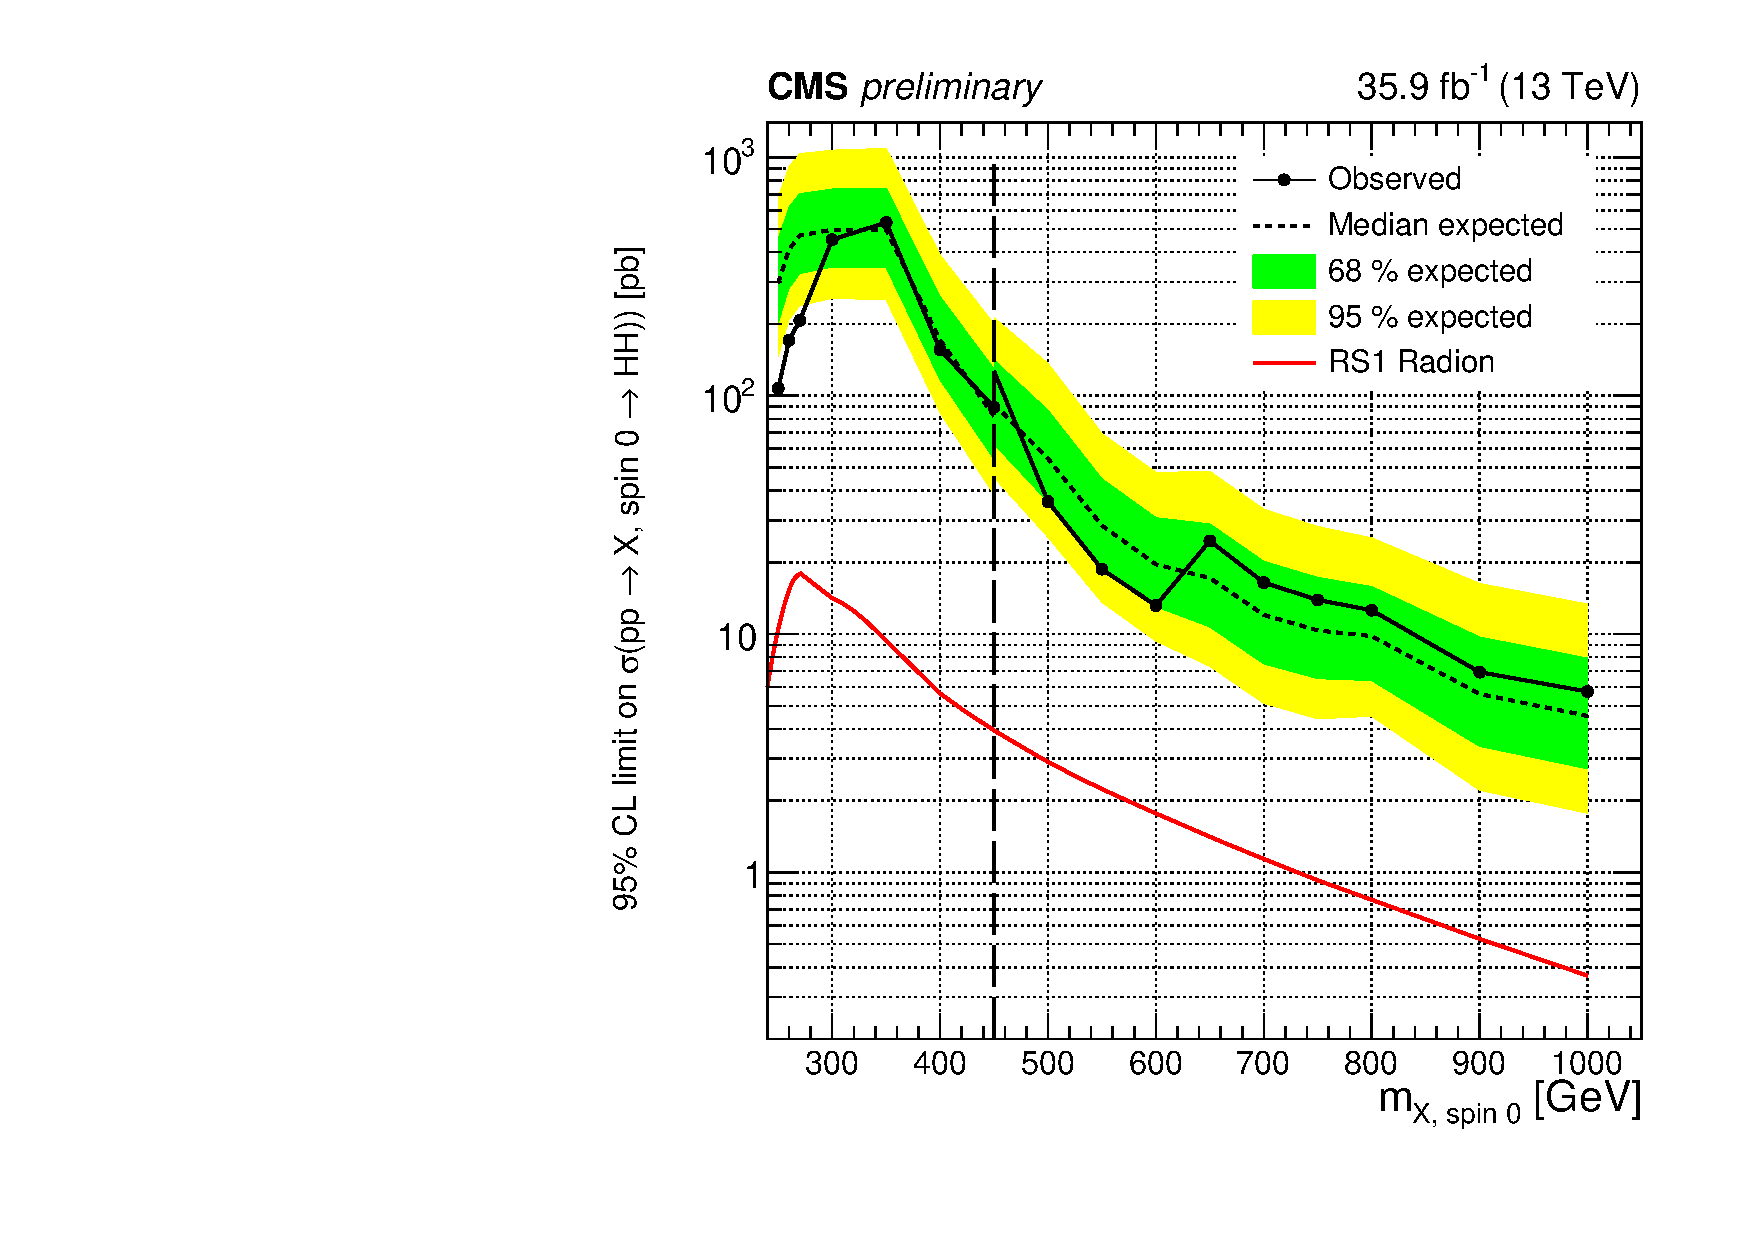
\includegraphics[width=0.65\textwidth]{limitHH_Nov16_radion.pdf}
    \caption{ Expected (dashed line) and observed (solid line) limits on the cross section of a resonant HH produ\
ction
      as a function of the mass of the narrow resonance for both leptonic channels combined. Graviton case is sho\
wn at the top and radion case at the bottom. The red line shows a theoretical prediction for
      the production of a WED particle with certain model assumptions \cite{Oliveira:2014kla}.
      }

      % Expected and observed limits on the HH production.                                                        
     %Top: in the 2 b jets, 2 lepton, 2 neutrinos final state optimized for the bbZZ selection. Bottom: full HH production.                                                                                                        

    \label{fig:HHlimits} %bbZZlimits                                                                              
  \end{center}
\end{figure}




%% \begin{table}
%% \begin{center}
%% \caption{Expected limits for full HH production. Combined data is used.}
%% \label{finalLimits}
%% \begin{tabular}{|c|c|}
%% %\toprule
%% \hline
%%  Mass, GeV &  Expected limit, pb \\\hline
%% %\midrule 
%%        260 &              220.62 \\
%%        270 &              241.75 \\
%%        300 &              248.25 \\
%%        350 &              116.25 \\
%%        400 &               49.97 \\
%%        450 &               28.38 \\
%%        600 &                6.91 \\
%%        650 &                5.73 \\
%%        900 &                2.41 \\
%%       1000 &                2.13 \\\hline

%% \end{tabular}
%% \end{center}
%% \end{table}


%added on april9
%% \begin{table}
%% \begin{center}
%% \caption{Expected limits for full HH production. Combined data is used.}
%% \label{finalLimits}
%% \begin{tabular}{|c|c|}
%% \hline
%%  Mass, GeV &  Expected limit, pb \\\hline
%% 260 & 240.62\\
%% 270 & 217.19\\
%% 300 & 296.09\\
%% 350 & 138.67\\
%% 400 & 66.99\\
%% %450 & 42.5\\
%% 450 & 32.27\\
%% 600 & 8.12\\
%% 650 & 6.33\\
%% 900 & 2.57\\
%% 1000 & 2.28\\\hline

%% \end{tabular}
%% \end{center}
%% \end{table}


%added on april26

%% \begin{table}
%% \begin{center}
%% \caption{Expected limits for full HH production. Combined data is used.}
%% \label{finalLimits}
%% \begin{tabular}{|c|c|c|}
%% \hline
%% Mass, GeV &  Expected limit, pb & Observed limit, pb \\\hline
%% 260.0 & 351.56 & 180.58 \\
%% 270.0 & 305.47 & 157.8 \\
%% 300.0 & 410.94 & 206.66 \\
%% 350.0 & 188.28 & 202.88 \\
%% 400.0 & 101.17 & 187.99 \\
%% 450.0 & 66.41 & 136.78 \\
%% 600.0 & 13.71 & 28.0 \\
%% 650.0 & 11.88 & 23.99 \\
%% 900.0 & 4.67 & 7.0 \\
%% 1000.0 & 4.22 & 6.96 \\\hline
%%\end{tabular}
%%\end{center}
%%\end{table}

%april27
%% \begin{table}
%% \begin{center}
%% \caption{Expected and observed limits for full HH production. Combined data is used.}
%% \label{finalLimits}
%% \begin{tabular}{|c|c|c|}
%% \hline
%% Mass, GeV &  Expected limit, pb & Observed limit, pb \\\hline
%% 260.0 & 351.6 & 180.6 \\
%% 270.0 & 305.5 & 157.8 \\
%% 300.0 & 410.9 & 206.7 \\
%% 350.0 & 188.3 & 202.9 \\
%% 400.0 & 101.2 & 188.0 \\
%% 450.0 & 66.4 & 136.8 \\
%% 600.0 & 13.7 & 28.0 \\
%% 650.0 & 14.1 & 25.8 \\
%% 900.0 & 4.7 & 7.0 \\
%% 1000.0 & 4.2 & 7.0 \\\hline
%% \end{tabular}
%% \end{center}
%% \end{table}




%april29
%% \begin{table}
%% \begin{center}
%% \caption{Expected limits for full HH production. Combined data is used.}
%% \label{finalLimits}
%% \begin{tabular}{|c|c|c|}
%% \hline
%% Mass, GeV &  Expected limit, pb & Observed limit, pb \\\hline
%% 260.0 & 351.6 & 180.6 \\
%% 270.0 & 305.5 & 157.8 \\
%% 300.0 & 410.9 & 206.7 \\
%% 350.0 & 188.3 & 202.9 \\
%% 400.0 & 101.2 & 188.0 \\
%% 450.0 & 66.4 & 136.8 \\
%% 600.0 & 13.7 & 28.0 \\
%% 650.0 & 11.9 & 24.0 \\
%% 900.0 & 4.7 & 7.0 \\
%% 1000.0 & 4.2 & 7.0 \\\hline
%% \end{tabular}
%% \end{center}
%% \end{table}




%june14
%% \begin{table}
%% \begin{center}                                                                                                                                            
%% \caption{Expected limits for full HH production. Combined data is used.}  
%% \label{finalLimits} 
%% \begin{tabular}{|c|c|} 
%% \hline
%%  Mass, GeV &  Expected limit, pb \\\hline
%%        250 &              264.06 \\
%%        260 &              309.38 \\
%%        270 &              318.75 \\
%%        300 &              418.75 \\
%%        350 &              210.16 \\
%%        400 &               92.58 \\
%%        450 &               52.15 \\
%%        500 &               33.91 \\
%%        550 &               18.98 \\
%%        600 &               14.57 \\
%%        650 &               12.15 \\
%%        700 &               11.33 \\
%%        750 &                9.65 \\
%%        800 &                7.66 \\
%%        900 &                5.96 \\
%%       1000 &                4.24 \\\hline
%% \end{tabular}
%% \end{center} 
%% \end{table}


%20july2018
%% \begin{table}
%% \begin{center}
%% \caption{Expected limits for full HH production. Combined data is used.}
%% \label{finalLimits}
%% \begin{tabular}{|c|c|}
%% \hline
%%  Mass, GeV &   Limit, pb \\
%% \hline
%%        250 &      253.5 \\
%%        260 &      272.2 \\
%%        270 &      274.4 \\
%%        300 &      380.0 \\
%%        350 &      330.6 \\
%%        400 &       90.4 \\
%%        450 &       59.8 \\
%%        451 &       87.1 \\
%%        500 &       31.0 \\
%%        550 &       14.5 \\
%%        600 &        9.8 \\
%%        650 &       18.5 \\
%%        700 &       16.1 \\
%%        750 &       13.7 \\
%%        800 &       10.1 \\
%%        900 &        8.1 \\
%%       1000 &        5.8 \\
%% \hline
%% \end{tabular}
%% \end{center}
%% \end{table}


%sept28
\begin{table}
\begin{center}
\caption{The expected and observed HH production cross section upper limits at 95\% CL for different
narrow resonance graviton (top) and radion (bottom) mass hypotheses for both dielectron and dimuon channels combined.}
\label{finalLimits}
\begin{tabular}{|c|c|c|}
%\toprule                                                                                                                                        
\hline
Mass, GeV &  Observed Limit, pb &  Expected Limit, pb \\
\hline
%\midrule                                                                                                                                        
      250 &               253.5 &               589.1 \\
      260 &               272.2 &               585.9 \\
      270 &               274.4 &               537.5 \\
      300 &               380.0 &               434.4 \\
      350 &               330.6 &               309.4 \\
      400 &                90.4 &               119.9 \\
      450 &                59.8 &                63.3 \\
      500 &                31.0 &                36.6 \\
      550 &                14.5 &                20.2 \\
      600 &                 9.8 &                12.7 \\
      650 &                18.5 &                11.1 \\
      700 &                16.1 &                10.1 \\
      750 &                13.7 &                 8.8 \\
      800 &                10.1 &                 6.5 \\
      900 &                 8.1 &                 4.8 \\
     1000 &                 5.8 &                 4.2 \\
%\bottomrule                                                                                                                                     
\hline
\end{tabular}
%% \end{center}                                                                                                                                  
%% \end{table}                                                                                                                                   
%% \begin{table}                                                                                                                                 
%% \begin{center}                                                                                                                                
%\caption{The expected and observed HH production cross section upper limits at 95\% CL for different narrow resonance Radion mass hypotheses for both dielectron and dimuon channels combined.}                                                                                                 
\vspace{1 cm} \ \\
%\label{tab:finalLimits}                                                                                                                         
\begin{tabular}{|c|c|c|}
%\toprule                                                                                                                                        
\hline
Mass, GeV &  Observed Limit, pb &  Expected Limit, pb \\
\hline
%\midrule                                                                                                                                        
     250.0 &               107.3 &               297.7 \\
     260.0 &               170.8 &               410.9 \\
     270.0 &               207.0 &               470.3 \\
     300.0 &               451.7 &               496.9 \\
     350.0 &               532.6 &               496.9 \\
     400.0 &               155.7 &               171.1 \\
     450.0 &                89.3 &                82.0 \\
     500.0 &                36.0 &                54.4 \\
     550.0 &                18.7 &                28.5 \\
     600.0 &                13.2 &                19.6 \\
     650.0 &                24.6 &                17.2 \\
     700.0 &                16.4 &                12.0 \\
     750.0 &                13.9 &                10.4 \\
     800.0 &                12.6 &                 9.8 \\
     900.0 &                 6.9 &                 5.6 \\
    1000.0 &                 5.7 &                 4.5 \\
%\bottomrule                                                                                                                                     
\hline
\end{tabular}
\end{center}
\end{table}


%For the HL-LHC none of the HH analyses can reach the discovery sensitivity, thus the goal for all HH analyses is to contribute to the grand combination and in this collaborative way to achieve the desired sensitivity. The most recent combination results for the spin 0 case are shown at the Fig. \ref{HH_combo}.



%% \begin{figure}[!htb]%hbpt?                                                                                                               
%% 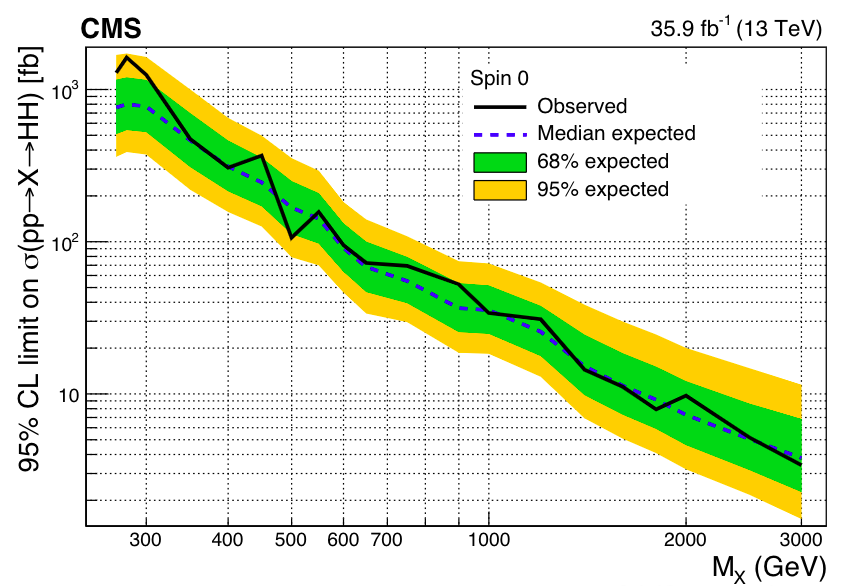
\includegraphics[width=0.5\textwidth, height=0.2\textheight,  keepaspectratio]{spin0_combo.png}
%% \caption{ The current combination of HH channels for the spin 0 heavy resonance hypothesis. }
%% \label{HH_combo}
%% \end{figure}









%% %added on dec17
%% \begin{table}
%% \begin{center}
%% \caption{Expected limits for full HH production. Combined data is used.}
%% \label{finalLimits}
%% \begin{tabular}{|c|c|}
%% \hline
%%  Mass, GeV &  Expected limit, pb \\\hline
%%       260 &              274.00 \\
%%        270 &              306.50 \\
%%        300 &              306.00 \\
%%        350 &              141.88 \\
%%        400 &               59.00 \\
%%        450 &               34.12 \\
%%        600 &                7.69 \\
%%        650 &                6.31 \\
%%        900 &                2.59 \\
%%       1000 &                2.25 \\\hline

%% \end{tabular}
%% \end{center}
%% \end{table}

